% REMEMBER: You must not plagiarise anything in your report. Be extremely careful.

\documentclass{l4proj}

    
%
% put any additional packages here
%

\begin{document}

%==============================================================================
%% METADATA
\title{Social Acceptability of Novel Interaction Techniques}
\author{Robert B. Thomson}
\date{November 03, 2020}

\maketitle

%==============================================================================
%% ABSTRACT
\begin{abstract}
    Every abstract follows a similar pattern. Motivate; set aims; describe work; explain results.
    \vskip 0.5em
    ``XYZ is bad. This project investigated ABC to determine if it was better. 
    ABC used XXX and YYY to implement ZZZ. This is particularly interesting as XXX and YYY have
    never been used together. It was found that  
    ABC was 20\% better than XYZ, though it caused rabies in half of subjects.''
\end{abstract}

%==============================================================================

% EDUCATION REUSE CONSENT FORM
% If you consent to your project being shown to future students for educational purposes
% then insert your name and the date below to  sign the education use form that appears in the front of the document. 
% You must explicitly give consent if you wish to do so.
% If you sign, your project may be included in the Hall of Fame if it scores particularly highly.
%
% Please note that you are under no obligation to sign 
% this declaration, but doing so would help future students.
%
%\def\consentname {My Name} % your full name
%\def\consentdate {20 March 2018} % the date you agree
%
\educationalconsent


%==============================================================================
\tableofcontents

%==============================================================================
%% Notes on formatting
%==============================================================================
% The first page, abstract and table of contents are numbered using Roman numerals and are not
% included in the page count. 
%
% From now on pages are numbered
% using Arabic numerals. Therefore, immediately after the first call to \chapter we need the call
% \pagenumbering{arabic} and this should be called once only in the document. 
%
% Do not alter the bibliography style.
%
% The first Chapter should then be on page 1. You are allowed 40 pages for a 40 credit project and 30 pages for a 
% 20 credit report. This includes everything numbered in Arabic numerals (excluding front matter) up
% to but excluding the appendices and bibliography.
%
% You must not alter text size (it is currently 10pt) or alter margins or spacing.
%
% 
%==================================================================================================================================
%
% IMPORTANT
% The chapter headings here are **suggestions**. You don't have to follow this model if
% it doesn't fit your project. Every project should have an introduction and conclusion,
% however. 
%
%==================================================================================================================================
\chapter{Introduction}

% reset page numbering. Don't remove this!
\pagenumbering{arabic}


\section{Overview}
Social acceptability plays an important role in a person's willingness to use and interact with technology [Rico2010, Ahlstrom2014]. Novel interaction modalities and new interactive devices may initially be perceived as socially unacceptable due to being unfamiliar and maybe even unusual to onlookers---especially if it is not clear that a person is using a computing device. The aim of this dissertation is to evaluate the social acceptability of novel interaction techniques for mobile devices, focusing on the use of gestures for input. Device motion gestures (e.g., shaking a phone) and contactless gestures (e.g., waving above the screen) are widely supported by modern smartphones, but are yet to be widely adopted by users, especially contactless gestures.

This work also investigates a new aspect of perceived social acceptability, looking at the relationship between social acceptability and perceptions of how \textit{useful} an interaction may be to a user. Perceived usefulness or benefit to a user could influence perceptions of social acceptability by attributing a clear reason for \textit{why} a person is interacting with a device in a certain way. How this usefulness changes with exposure and familiarity will also be explored (e.g., to see if interactions become more acceptable as users begin to recognise their benefits).

The research begins with a preliminary survey to investigate current opinions on the use of novel interaction techniques and devices. Following this, an Android media player, with incorporated gesture input, was created. User evaluations over the course of one week were used to analyse the effect of using the novel interaction for the purpose of musical enjoyment over a period of time. Observations are made..... And conclusions are drawn.....


\section{Motivation}
Technological advances mean people are interacting in more ways with an increasing number of devices on a daily basis. In turn, people become more and more reliant on new devices and interaction modalities, because they offer more convenient ways of accessing services and information. They can be very efficient at helping us complete tasks in our everyday lives. 

People can often feel that using novel interaction techniques is socially unacceptable (i.e., that their use would be perceived negatively by other people). This is a serious issue for interaction designers and device manufacturers, as negative perceptions may slow down or prevent the adoption of new technologies. If an interaction is not deemed socially acceptable or does not adhere to social norms, the product seems likely to fail. Very few people will be happy to use it in their day to day lives if it might attract unwanted attention or negative perceptions from others.  It is often just taken for granted that if interaction is too different from the current technologies, or has an unclear use case, then the population will not get behind it. For example, Google Glass was negatively affected by lack of acceptance due to perceived privacy concerns, because interactions with the system and its intended applications were unclear.

Social acceptability is largely affected by the location of use and the `audience' of an interaction [Rico]. This is likely the case for certain circumstances of interactions. However, I believe that a persons familiarity with an interaction method will have just as large an impact, if not more, than these factors on their perceptions of acceptability. I believe the perceived use of an interaction technique will grow over time. As a result, the user may be more likely to perceive it to be socially acceptable. Possible factors of how quickly and likely these changes to perception are to occur are (1)~how useful a technique is and (2)~how little effort is required to use it, in comparison to the standard method of completing the desired task. These factors will be explored through this work.

\section{Aims}
In response to this motivation, requirements will be gathered through the use of a user survey. This will provide an initial outlook of participants views on social norms and stigmas around effort and usefulness. It will expose how usefulness effects how participants they currently use the novel interaction techniques in question. Namely; gesture input, smart glasses (specifically Snapchat Spectacles) and voice assistant interactions. 

Following the gathering of requirements, a media player is implemented with integrated motion gesture input potential. Participants will be asked to use the mobile app for a period of time and they will be interviewed at various stages. The hope in doing this, is that it will show that users become familiar with the method of interaction over the time period. It is hypothesised that participants will find it more useful and easier to use with time and in turn believe it to become socially acceptable in more situations. It is believed that this will provide researchers with a new outlook on social acceptability, the context of a situation is the boundary that must be met socially but it is determined by the users perceived usefulness and familiarity of an interaction method. It is hoped that interaction designers and product manufactures will use the conclusions to aim to make interaction techniques that are easy to familiarise ones self with, as opposed to being completely socially acceptable "out of the box". 
\section{Limitations}
With a focus on COVID-19. Possibly at the end ?


%==================================================================================================================================
\chapter{Background Research and Related Works}
\section{Overview}
The research has been on the building block of many others from various areas. Background research of these areas was conducted extensively to develop the ideas and aims of this paper. What defines a novel interaction  was first investigated to validate my knowledge of such technology. The interactions and social acceptability of these devices were then explored in more detail. Finally, social norms around usefulness and effort were delved into more deeply.
\section{Novel Interactions}

In simple terms, an interaction with a device can be described as and action in which a users communicates input to the device, when the device provides output to the user or a combination of both through interfaces. In the field of Human Computer Interaction it is taken to be more of the way one experiences using the device and their perception of it[...Designing Interactions]. These interactions can use various techniques and are said to be novel when they are not commonly used or new to the users of the devices. These interactions can be through various parts of the device or completely encompass the device itself. 

Various pieces of literature have set guidelines for how interfaces and interactions should be designed [Guidelines...&designing interactions]. However, guidelines and practices change very regularly. There has always been an attention on invisible interfaces for personal use[...really really]. These prospects will be built on to understand how the effort required to interact dictates the invisibility and if this invisibility relates to how users feel others will perceive them in social situations.

\section{Social Acceptability}

Individuals make decisions on the social acceptability of tasks on a daily basis. They do by using their existing knowledge to assess their surroundings and consider the action to determined if it would be deemed acceptable [presentation of self...]. This is done when interacting with technology. Users evaluate their motivations and desire to use the technology and compare this to the restrictions of social normality's. This is important of manufacturers and designers as if a product or interaction technique is perceived to be socially unacceptable users will not be willing to use them and they will fail.

There are some widely given structures of how social acceptability of a device can be assessed. These will be considered and built on but a slightly different approach will be taken. Rico et al.[....]. suggested that users see the interaction as a performance that must be done appropriately in various contexts. For example ones performance must not be done too noticeably in some contexts whereas in others there is more of a focus on doing the performance correctly. Ahlstrom et al.[...]. explored the possibility of introversion or extroversion traits playing a part in what a user deems acceptable. For example the users personality can be what deems a task and its motivation acceptable in a given set of surroundings. An approach slightly more in line with Occam's razor is given by Sakamoto et al.[...]. where it is believed that a users aim when interacting is simply not to be noticed. This paper will take the stance that users will be comfortable using an interaction method if they believe they will be perceived as not putting in too much effort with respect to the outcome. Therefore, in turn, as a user gains experience achieving the usefulness of an interaction method, the more socially acceptable they will perceive it to be due to its enhanced invisibility.

\subsection{Voice Assistants}

Voice assistants, like the Amazon Echo and Google Nest, are new and innovative devices that primarily make use of Voice User Interfaces. VUIs are an interaction technique that have divided many people. This is often due to their range of potential uses, reliability and acceptability. Issues with reliability often mean that, following attempts to control the device with their voice, they have to fall back to interacting with it through their mobile device. This means much more effort is needed to be used than simply talking to it, which can even itself be seen to not be as easy as just interacting with it with ones phone in the first place. This makes the user frustration for the device and reduces their confidence in using it. This lack of confidence could be brought about by the VUI being socially unacceptable to try so hard to interact with and become frustrated at. This impact on acceptability has been under investigated.

Picture?

A Common method of gathering data about peoples views of a Voice Assistant is by analysing online product reviews. Experimental methods of this nature alone may not give a clear picture of the population as only certain groups of users may feel the need to leave a review, skewing the results. This was done in an attempt to find users satisfaction and personification of the Amazon Echo [BFF...]. Some results that the authors were not directly looking for were found. It was identified that if technical errors were experienced that users were reluctant to continue using the device. It was assumed that this lack of invisibility caused people to not want to have to go to the bother of using it again. However this report will explore the potential that technical issues require additional effort that people do not want to appear to have to make as it may show that they are incapable of achieving the uses of the interaction method easily.

A lab study undertaken by Myers et al.[Patterns...] investigated the causes and impacts of the frustration caused by VUIs. The experiment involved participants interacting with the device in a laboratory setting and required them to undertake set tasks on three occasions. Common errors made by participants were recorded and their levels of frustration. Users didn't take notice of times when the device accepted their attempts to interact indicating it achieved invisibility and had the potential to be acceptable. However when users had to put extra effort in they became annoyed and when it reoccurred in later occasions their frustration was reinforced. The acceptability of this reduced usefulness was not examined and could be explored in this research as being frustrated is rarely seen as acceptable in other aspects of life. The Lab setting and set tasks limited these results as conclusions may not be strongly valid for how users would use the interaction techniques in the wild.

Myers et al.[Impact...] build on their previous work by exploring the limitations of the invisible nature of VUIs. Online responses and reviews were examined and an in the wild experiment were carried out in the hope of making in more Ecologically valid in comparison to the previous work. This dual method will be attempted in this study of interaction methods as both together can be ecologically valid by being in the wild while also gaining responses from large numbers of participants which may not have been possible to achieve due to the nature of using an interaction technique for an extended time.

From this investigation of Voice assistants, it is clear that previous literature has aimed to find how people use Voice assistants. The reasons people may avoid using them have either not been explored, or been found by accident during analysis. This study will focus on the social reasons users may avoid using different novel interaction techniques through a combination of different experimental methods used by the above literature.

\subsection{Gestures}

What is a Gesture
A Gesture can be described as a communication form that is non-verbal. This is said to be hand movements. In the case of device interaction a gestures have three main categories, each of which will be explored. The most common form is touch screen gestures. These are things like using multiple fingers, using varying pressures or making certain shapes to interact with the devices touch screen. This is widely used by many devices and applications and is generally accepted but users. Device Motion Gestures and Mid-Air Gestures are the other two main categories of Gesture but are used and advertised buy device and application producers. This is likely due to the invisibility of touch screen gestures to the public around the user and the perceived lack there of for other gestures. 

Picture?

The majority of previous literature has focused on gestures as not being socially acceptable on particular locations or in certain companies [Rico...]. This is generally assessed by asking a participant to carry out various tasks in the wild. The participants views are either recorded throughout the tasks[are you comfortable ...] or collected at the end using an interview[...rico]. Users can also be examined on various metrics to understand how well they carry out the gesture[Rhythmic...]. Freeman et al.[...] detailed that mid air gestures were very usable and completed easily when users were given instruction and found audio signals aligned well with their use due to the consistent eyes free nature of the features. This provides ground for the opportunity that users will be able to get more used to and more easily gain the benefits of Mid-Air Gestures. This will be explored with respect the the perceived social acceptance that is brought along with it.

Where gestures are performed is the focus of the study done by Rico et al. [...]. The author describes various types of gesture and explains why some of them are reasonable or should not be used. It is suggested that optimal gestures should mimic gestures that people may come across in their everyday life as they can be more familiar. Gestures that are found not to be effective are of an emblematic style as these may have preexisting meanings and could therefore be confused for their established connotations. Analysis will be done to maintain and solidify that using familiar gestures will make it easier for users to get used to using them, increasing their usefulness and therefore social acceptability.

Acceptance of an interaction method has also been found to have a strong correlation to where, with respect to their body, the user performs a gesture. Ahlström et al.[...] found that if carrying out the gesture took more than 6 seconds, the user tends to not see it as acceptable. The same stands for if the gesture requires the user to move more than a foot away from the device. Ahlström et al. [...] believe this to be purely for visual reasons as it may look unnatural to others. However this could indicate that users perceive an interaction technique to be socially unacceptable if they believe others around them will perceive them to be putting in an abnormal amount of effort to interact. This will be explored and strengthened through experimental analysis.

\subsection{Smart Glasses}

A wearable device is a broad term that covers devices such as Smart Glasses, Watches and Rings. Since these devices take the place of common fashion accessories they have an inherent need to be social acceptable. They must be  aesthetically pleasing, up to date with current trends and comfortable, all while facing the same interaction challenges of other devices, systems and applications. This study will focus only on the interactions with these types of devices, in particular Smart Glasses.

Research carried out by Chuah et al. [...] attempts to understand the factors that determine the widespread adoption of smartwatches by the population. It was concluded that visibility and perceived usefulness are large factors in this adoption. This will be explored to establish if it is due to the user wanting to appear visible and not using effort 
by others which makes them confident in using the devices - and similarly other novel interaction techniques - in social situations. Other studies focused on smart glasses are in appearance that a device and its interaction modalities being unobtrusive enhance its social acceptance. This will be elaborated to understand if this is common for other interaction techniques and to decide if, over time, users will better understand interaction techniques to become more comfortable using them, even if they are slightly obtrusive, due to a new found familiarity.

The Focus of this area of study will be directed towards the social acceptability and the use fullness of the Snapchat Spectacles as the product was available to me. The product and its interaction methods have been vastly speculated in the technical community [...Article?WhyDidTheyFail]. It is often deemed that the product was a failure and never took off. It seems that even when people bought the device, they rarely used it consistently and often stopped using it after as little as a week [...ArticleWhySnapchatSpectaclesFailed]. At this time there have been 3 iterations of the Spectacles and none of them have been close to being a common household item. The general consensus is that the fear brought about by other data glasses[...Don't Look at me].

Picture?


\section{Effort, Usefulness and Acceptability}

Perceived usefulness and effort required are is strongly linked. When solving an immediate problem, one will view it in comparison to their background of probable future problems[Human behaviour...].  If an individual sees an outcome as having less worth than the effort required to conduct the required task, it is likely they will not see it as useful and not want to do it . Kingsley also suggests that it is the socilal norm that a person will strive to expend the least amount of energy to solve a problem. In terms of using novel interaction techniques this can be translated to if the input to a device requires more energy than what the desired output is worth, they will not want to do it. Other literature [...perceived usefulness] strongly backs up this case in the context of personal user acceptance and has set guidelines to do so. Kingsley also believes that, "A person is socially treated according to the social signals he emits". This together with social norms of least effort, it will be explored if one has a concern that not only do they want to reduce effort to conserve energy, but also so it does not appear to others that they are wasting it. 

This claim is again backed up extracting knowledge from a study of attitudes among students[Student...]. If one wants to be accepted by society, they must give off the correct norm of socially signals accordingly. In this study it is found that from a young age, we learn that the social norm is to put in the least viable amount of effort. Therefore to be a part of the social norm we must adhere to this and not be seen to put in any effort or only as little as possible. Social signals coming from the effort expelled when providing input through novel interaction techniques will be explored to understand if this is common among these circumstances. It will be decided if invisibility of effort expelled is what is socially desirable, the same way it is when using a system to complete tasks for ones personal needs.

These implications will be analysed in the case of other novel interaction techniques and their social implications will be explored over time. It is thought that the more a user makes use of an interaction method, two main things may happen and will be observed. The users will become more used to using the device and feel as though the desired outcome requires less effort and become more useful. Additionally, they may come across more more useful functions that were not evident before use, increasing the output they will get by using it meaning it is acceptable to use more effort. These together will imply that a user will perceive the task to become more useful over time and and less effort in comparison will be expelled, making it more socially acceptable to do. Acceptance growing over time is examined in detail in The walkman effect[...]. This study details how over time as people use or do something it will gradually become more normal to do. The populations initial attitude towards the walkman was largely negative as it was a very out of the ordinary thing to use or be seen using. However, over time people became more attuned to it as its usefulness and ease of use that they became much more accepting to it as more and more others accepted it. Before long it became a norm. This effect will be investigated to understand if the same stands for novel interaction techniques.



%==================================================================================================================================
\chapter{Requirements Gathering}

\section{Outline}

\section{User Survey
}
\subsection{Methodology}

\subsection{Results}

%==================================================================================================================================
\chapter{Technical Development}
brief summary of development
\section{Platform}
Talk about the platforms considered to produce something. Android studio, spotify sdk, Google Home smart home action? Why was what was chosen done so(reasoning).
\section{Process}
Overview of how the app was created
\subsection{Programming}
What was developed, issues and how they were overcome
\subsection{Gestures}
How the gestures were decided and why. How they were created, why were they created that way.
\subsection{Assets}
How music was ethically and legally found, possible repercussions avoided
\section{Testing}
Tests that were undergone and why


%==================================================================================================================================

\chapter{Experiment Design}

\section{Outline}

\section{User Evaluation Design}

%==================================================================================================================================

\chapter{User Evaluation}

\section{Methodology}

\section{Results}

%==================================================================================================================================
\chapter{Evaluation} 

\section{Usage change}

\section{User Perceptions}

\section{Evidence}

%==================================================================================================================================
\chapter{Conclusion}  
\section{Implications}
Summarise the whole project for a lazy reader who didn't read the rest (e.g. a prize-awarding committee).
\section{Future Work}


%==================================================================================================================================
\chapter{General Guidelines}

These points apply to the whole dissertation.

\subsection{Figures}
\emph{Always} refer to figures included, like Figure \ref{fig:relu}, in the body of the text. Include full, explanatory captions and make sure the figures look good on the page.
You may include multiple figures in one float, as in Figure \ref{fig:synthetic}, using \texttt{subcaption}, which is enabled in the template.



% Figures are important. Use them well.
\begin{figure}
    \centering
    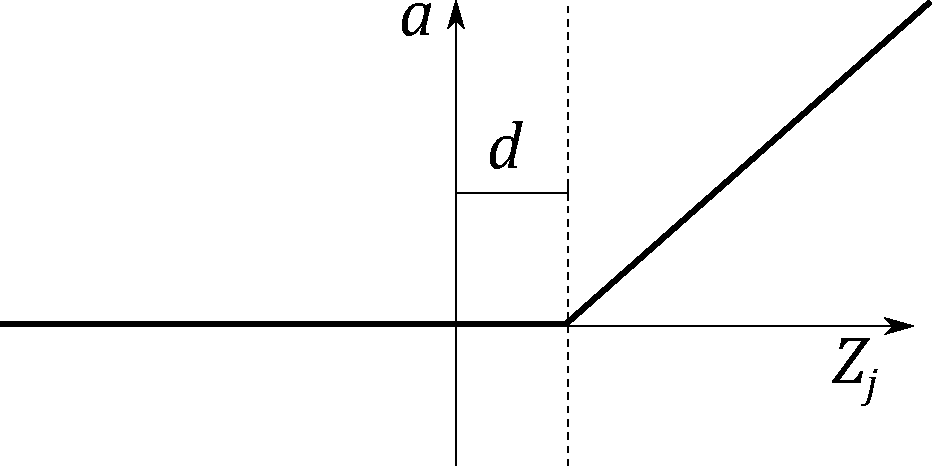
\includegraphics[width=0.5\linewidth]{images/relu.pdf}    

    \caption{In figure captions, explain what the reader is looking at: ``A schematic of the rectifying linear unit, where $a$ is the output amplitude,
    $d$ is a configurable dead-zone, and $Z_j$ is the input signal'', as well as why the reader is looking at this: 
    ``It is notable that there is no activation \emph{at all} below 0, which explains our initial results.'' 
    \textbf{Use vector image formats (.pdf) where possible}. Size figures appropriately, and do not make them over-large or too small to read.
    }

    % use the notation fig:name to cross reference a figure
    \label{fig:relu} 
\end{figure}


\begin{figure}
    \centering
    \begin{subfigure}[b]{0.45\textwidth}
        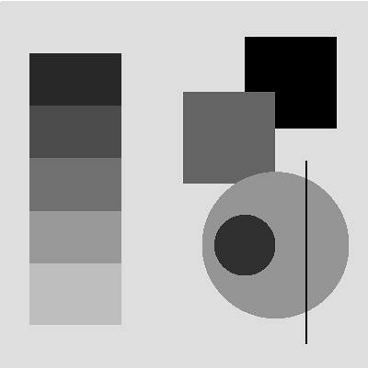
\includegraphics[width=\textwidth]{images/synthetic.png}
        \caption{Synthetic image, black on white.}
        \label{fig:syn1}
    \end{subfigure}
    ~ %add desired spacing between images, e. g. ~, \quad, \qquad, \hfill etc. 
      %(or a blank line to force the subfigure onto a new line)
    \begin{subfigure}[b]{0.45\textwidth}
        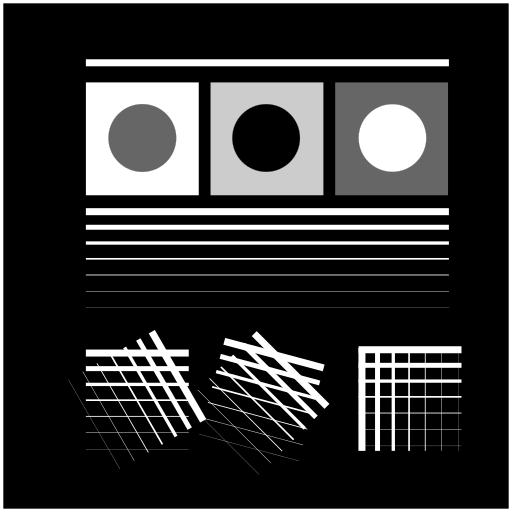
\includegraphics[width=\textwidth]{images/synthetic_2.png}
        \caption{Synthetic image, white on black.}
        \label{fig:syn2}
    \end{subfigure}
    ~ %add desired spacing between images, e. g. ~, \quad, \qquad, \hfill etc. 
    %(or a blank line to force the subfigure onto a new line)    
    \caption{Synthetic test images for edge detection algorithms. \subref{fig:syn1} shows various gray levels that require an adaptive algorithm. \subref{fig:syn2}
    shows more challenging edge detection tests that have crossing lines. Fusing these into full segments typically requires algorithms like the Hough transform.
    This is an example of using subfigures, with \texttt{subref}s in the caption.
    }\label{fig:synthetic}
\end{figure}

\clearpage

\subsection{Equations}

Equations should be typeset correctly and precisely. Make sure you get parenthesis sizing correct, and punctuate equations correctly 
(the comma is important and goes \textit{inside} the equation block). Explain any symbols used clearly if not defined earlier. 

For example, we might define:
\begin{equation}
    \hat{f}(\xi) = \frac{1}{2}\left[ \int_{-\infty}^{\infty} f(x) e^{2\pi i x \xi} \right],
\end{equation}    
where $\hat{f}(\xi)$ is the Fourier transform of the time domain signal $f(x)$.

\subsection{Algorithms}
Algorithms can be set using \texttt{algorithm2e}, as in Algorithm \ref{alg:metropolis}.

% NOTE: line ends are denoted by \; in algorithm2e
\begin{algorithm}
    \DontPrintSemicolon
    \KwData{$f_X(x)$, a probability density function returing the density at $x$.\; $\sigma$ a standard deviation specifying the spread of the proposal distribution.\;
    $x_0$, an initial starting condition.}
    \KwResult{$s=[x_1, x_2, \dots, x_n]$, $n$ samples approximately drawn from a distribution with PDF $f_X(x)$.}
    \Begin{
        $s \longleftarrow []$\;
        $p \longleftarrow f_X(x)$\;
        $i \longleftarrow 0$\;
        \While{$i < n$}
        {
            $x^\prime \longleftarrow \mathcal{N}(x, \sigma^2)$\;
            $p^\prime \longleftarrow f_X(x^\prime)$\;
            $a \longleftarrow \frac{p^\prime}{p}$\;
            $r \longleftarrow U(0,1)$\;
            \If{$r<a$}
            {
                $x \longleftarrow x^\prime$\;
                $p \longleftarrow f_X(x)$\;
                $i \longleftarrow i+1$\;
                append $x$ to $s$\;
            }
        }
    }
    
\caption{The Metropolis-Hastings MCMC algorithm for drawing samples from arbitrary probability distributions, 
specialised for normal proposal distributions $q(x^\prime|x) = \mathcal{N}(x, \sigma^2)$. The symmetry of the normal distribution means the acceptance rule takes the simplified form.}\label{alg:metropolis}
\end{algorithm}

\subsection{Tables}

If you need to include tables, like Table \ref{tab:operators}, use a tool like https://www.tablesgenerator.com/ to generate the table as it is
extremely tedious otherwise. 

\begin{table}[]
    \caption{The standard table of operators in Python, along with their functional equivalents from the \texttt{operator} package. Note that table
    captions go above the table, not below. Do not add additional rules/lines to tables. }\label{tab:operators}
    %\tt 
    \rowcolors{2}{}{gray!3}
    \begin{tabular}{@{}lll@{}}
    %\toprule
    \textbf{Operation}    & \textbf{Syntax}                & \textbf{Function}                            \\ %\midrule % optional rule for header
    Addition              & \texttt{a + b}                          & \texttt{add(a, b)}                                    \\
    Concatenation         & \texttt{seq1 + seq2}                    & \texttt{concat(seq1, seq2)}                           \\
    Containment Test      & \texttt{obj in seq}                     & \texttt{contains(seq, obj)}                           \\
    Division              & \texttt{a / b}                          & \texttt{div(a, b) }  \\
    Division              & \texttt{a / b}                          & \texttt{truediv(a, b) } \\
    Division              & \texttt{a // b}                         & \texttt{floordiv(a, b)}                               \\
    Bitwise And           & \texttt{a \& b}                         & \texttt{and\_(a, b)}                                  \\
    Bitwise Exclusive Or  & \texttt{a \textasciicircum b}           & \texttt{xor(a, b)}                                    \\
    Bitwise Inversion     & \texttt{$\sim$a}                        & \texttt{invert(a)}                                    \\
    Bitwise Or            & \texttt{a | b}                          & \texttt{or\_(a, b)}                                   \\
    Exponentiation        & \texttt{a ** b}                         & \texttt{pow(a, b)}                                    \\
    Identity              & \texttt{a is b}                         & \texttt{is\_(a, b)}                                   \\
    Identity              & \texttt{a is not b}                     & \texttt{is\_not(a, b)}                                \\
    Indexed Assignment    & \texttt{obj{[}k{]} = v}                 & \texttt{setitem(obj, k, v)}                           \\
    Indexed Deletion      & \texttt{del obj{[}k{]}}                 & \texttt{delitem(obj, k)}                              \\
    Indexing              & \texttt{obj{[}k{]}}                     & \texttt{getitem(obj, k)}                              \\
    Left Shift            & \texttt{a \textless{}\textless b}       & \texttt{lshift(a, b)}                                 \\
    Modulo                & \texttt{a \% b}                         & \texttt{mod(a, b)}                                    \\
    Multiplication        & \texttt{a * b}                          & \texttt{mul(a, b)}                                    \\
    Negation (Arithmetic) & \texttt{- a}                            & \texttt{neg(a)}                                       \\
    Negation (Logical)    & \texttt{not a}                          & \texttt{not\_(a)}                                     \\
    Positive              & \texttt{+ a}                            & \texttt{pos(a)}                                       \\
    Right Shift           & \texttt{a \textgreater{}\textgreater b} & \texttt{rshift(a, b)}                                 \\
    Sequence Repetition   & \texttt{seq * i}                        & \texttt{repeat(seq, i)}                               \\
    Slice Assignment      & \texttt{seq{[}i:j{]} = values}          & \texttt{setitem(seq, slice(i, j), values)}            \\
    Slice Deletion        & \texttt{del seq{[}i:j{]}}               & \texttt{delitem(seq, slice(i, j))}                    \\
    Slicing               & \texttt{seq{[}i:j{]}}                   & \texttt{getitem(seq, slice(i, j))}                    \\
    String Formatting     & \texttt{s \% obj}                       & \texttt{mod(s, obj)}                                  \\
    Subtraction           & \texttt{a - b}                          & \texttt{sub(a, b)}                                    \\
    Truth Test            & \texttt{obj}                            & \texttt{truth(obj)}                                   \\
    Ordering              & \texttt{a \textless b}                  & \texttt{lt(a, b)}                                     \\
    Ordering              & \texttt{a \textless{}= b}               & \texttt{le(a, b)}                                     \\
    % \bottomrule
    \end{tabular}
    \end{table}
\subsection{Code}

Avoid putting large blocks of code in the report (more than a page in one block, for example). Use syntax highlighting if possible, as in Listing \ref{lst:callahan}.

\begin{lstlisting}[language=python, float, caption={The algorithm for packing the $3\times 3$ outer-totalistic binary CA successor rule into a 
    $16\times 16\times 16\times 16$ 4 bit lookup table, running an equivalent, notionally 16-state $2\times 2$ CA.}, label=lst:callahan]
    def create_callahan_table(rule="b3s23"):
        """Generate the lookup table for the cells."""        
        s_table = np.zeros((16, 16, 16, 16), dtype=np.uint8)
        birth, survive = parse_rule(rule)

        # generate all 16 bit strings
        for iv in range(65536):
            bv = [(iv >> z) & 1 for z in range(16)]
            a, b, c, d, e, f, g, h, i, j, k, l, m, n, o, p = bv

            # compute next state of the inner 2x2
            nw = apply_rule(f, a, b, c, e, g, i, j, k)
            ne = apply_rule(g, b, c, d, f, h, j, k, l)
            sw = apply_rule(j, e, f, g, i, k, m, n, o)
            se = apply_rule(k, f, g, h, j, l, n, o, p)

            # compute the index of this 4x4
            nw_code = a | (b << 1) | (e << 2) | (f << 3)
            ne_code = c | (d << 1) | (g << 2) | (h << 3)
            sw_code = i | (j << 1) | (m << 2) | (n << 3)
            se_code = k | (l << 1) | (o << 2) | (p << 3)

            # compute the state for the 2x2
            next_code = nw | (ne << 1) | (sw << 2) | (se << 3)

            # get the 4x4 index, and write into the table
            s_table[nw_code, ne_code, sw_code, se_code] = next_code

        return s_table

\end{lstlisting}

See the file \texttt{guide\_to\_visualising.pdf} for further information and guidance.

\begin{figure}
    \centering
    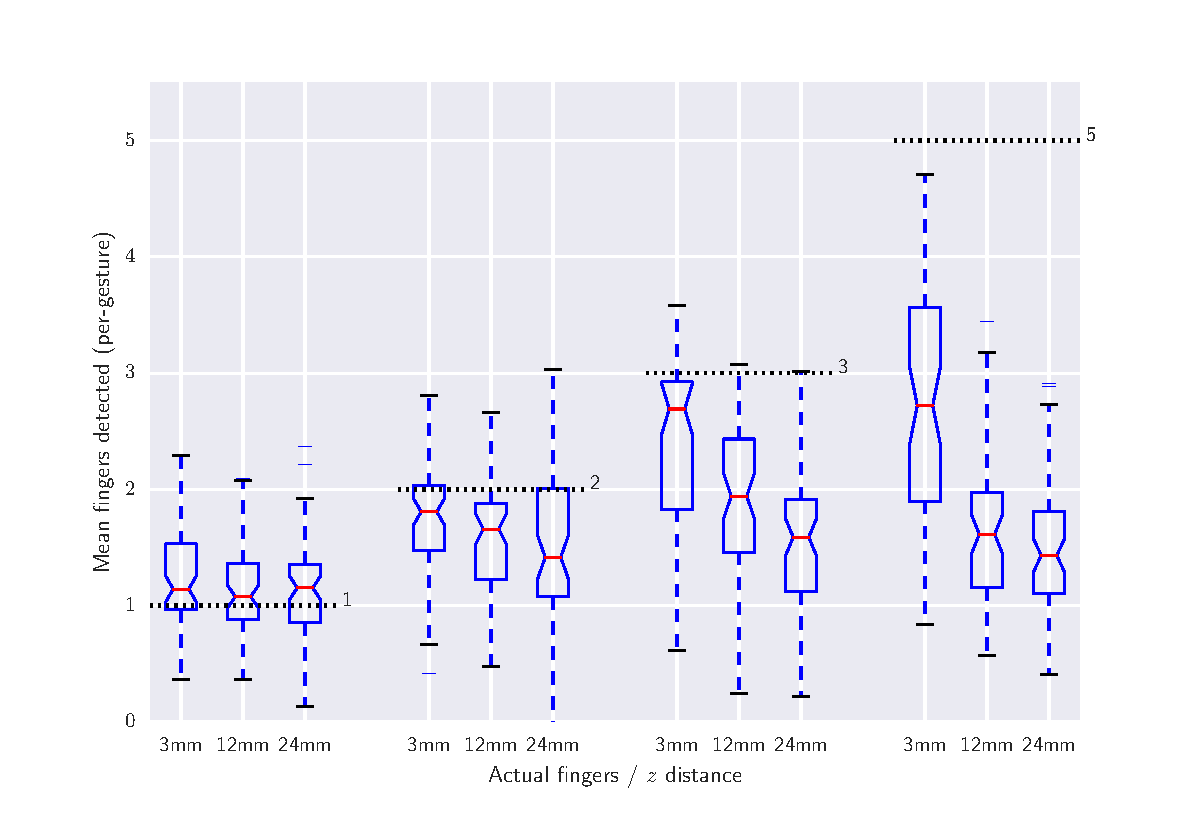
\includegraphics[width=1.0\linewidth]{images/boxplot_finger_distance.pdf}    

    \caption{Average number of fingers detected by the touch sensor at different heights above the surface, averaged over all gestures. Dashed lines indicate
    the true number of fingers present. The Box plots include bootstrapped uncertainty notches for the median. It is clear that the device is biased toward 
    undercounting fingers, particularly at higher $z$ distances.
    }

    % use the notation fig:name to cross reference a figure
    \label{fig:boxplot} 
\end{figure}


% 
%==================================================================================================================================
%  APPENDICES  
\begin{appendices}

\chapter{Appendices}

Typical inclusions in the appendices are:

\begin{itemize}
\item
  Copies of ethics approvals (required if obtained)
\item
  Copies of questionnaires etc. used to gather data from subjects.
\item
  Extensive tables or figures that are too bulky to fit in the main body of
  the report, particularly ones that are repetitive and summarised in the body.

\item Outline of the source code (e.g. directory structure), or other architecture documentation like class diagrams.

\item User manuals, and any guides to starting/running the software.

\end{itemize}

\textbf{Don't include your source code in the appendices}. It will be
submitted separately.

\end{appendices}

%==================================================================================================================================
%   BIBLIOGRAPHY   

% The bibliography style is abbrvnat
% The bibliography always appears last, after the appendices.

\bibliographystyle{abbrvnat}

\bibliography{l4proj}

\end{document}
